\documentclass{aa}
\usepackage[varg]{txfonts}
\usepackage{siunitx}
\usepackage[version=3]{mhchem}

\sisetup{
%     fixed-exponent      = 3,
%     list-units          = brackets,
    range-units         = brackets,
%     scientific-notation = fixed
}


\def\eps{\varepsilon}
\def\aap{A\&A}
\def\apj{ApJ}
\def\apjs{ApJS}
\def\apjl{ApJL}
\def\mnras{MNRAS}
\def\aj{AJ}
\def\nat{Nature}
\def\aaps{A\&A Supp.}
\def\prd{Phys. Rev. D}
\def\prl{Phys. Rev. Lett.}
\def\araa{ARA\&A}       % Annual Review of Astron and Astrophys

\begin{document}


\title{NIR spectroscopy of the Sun and HD20010}
\subtitle{Compiling a new linelist in the NIR}

\subtitle{}

\author{D.~T.~Andreasen\inst{1,2,3}
    \and N.~C.~Santos.\inst{1,2}
    \and S.~G.~Sousa.\inst{1,2}
    \and E.~Delgado Mena.\inst{1,2}}


\institute{
Centro de Astrof\'isica, Universidade do Porto, Rua das Estrelas,
4150-762, Porto, Portugal
    \email{daniel.andreasen@astro.up.pt}
\and
Instituto de Astrof\'isica e Ci\^encias do Espa\c{c}o, Universidade do Porto, CAUP, Rua das
Estrelas, PT4150-762 Porto, Portugal
\and
Departamento de F\'isica e Astronom\'ia, Faculdade de Ci\^encias, Universidade do Porto, Portugal
}







\date{\today}

\abstract{}{}{}{}



\keywords{data reduction: high resolution spectra -- data reduction: low
    resolution spectra -- stars individual: HD20010 -- stars individual: Sun}
\maketitle



\section{Introduction}
\label{sec:introduction}
Effective surface temperature ($T_\mathrm{eff}$), surface gravity ($\log g$),
and metallicity ([Fe/H], where iron is used as a proxy) are fundamental
atmospheric parameters necessary to characterise a star, as well to determine
other inderict fundamental parameters, such as mass, radius, and age from
stellar evolutionary models \citep{Girardi2000}.

Precise and accurate stellar parameters are also essential in exoplanet
searches. Planetary radius, and mass are mainly found from lightcurve
analysis and radial velocity analysis, respectively. These parameters
are related to the stellar parameters.

Today there are several methods of determine atmospheric parameters.
Interferometry of bright stars give highly accurate radii and effective
temperatures with low uncertainties. See e.g. \cite{Boyajian2012} for
application of interferometry of K and M stars. A newer technique
is asteroseismology were stellar pulsation observed at the surface
penetrates the interior of a star, and then reveals the inner structure.
From asteroseismology it is possible to relatively easy measure the
surface gravity and mean density, and therefore from scaling relations
\citep{Kjeldsen1995} calculate the mass and radius. This technique
have been tested in great extent for solar like stars and red giants
since the launch of the \emph{Kepler} mission and the CoRoT mission
\citep{Michel2008,Huber2011,Huber2012}.

From photometry we can find effective temperatures from simple color
relations. Such relations have been examined in \cite{Ramirez2005a} and
is a well known method. Yet another method is the infrared flux method
(IRFM) first described by \cite{Blackwell1977} and a newer study by
\cite{Ramirez2005b,Casagrande2010}. For this method, we need to know the
bolometric flux, surface gravity, and the metallicity a priori.
















\section{The method}
\label{sec:the_method}

Generally speaking there are two methods for determining parameters from
a spectrum. One is the spectral synthesis method, where a synthetic
spectrum is compared with an observed spectrum and by minimization
procedure the best fit is found between the synthetic spectrum and the
real spectrum \citep[see e.g.][]{Onehag2012}. The final atmospheric
parameters are found when the minimization procedure reach a minimum.

The other method is the equivalent width (EW) method, which we use in this
work.  With this method the EW are measured for all lines in a line list. The
EW is given as
\begin{align}
    \label{eq:EW}
    EW = \int_0^\infty \left(1 - \frac{F_\lambda}{F_0}\right) d\lambda,
\end{align}
where $F_0$ is the continuum level and $F_\lambda$ is the flux as a function
of wavelength. In other words, the EW is the area from a spectral line up
to the normalized continuum level.

With the EW method abundance for individual lines can be found with a code like
MOOG\footnote{The MOOG code can be downloaded free at
\url{http://www.as.utexas.edu/~chris/moog.html}}. By changing atmospheric
parameters as input for MOOG, similar abundances will be achieved for similar
elements when the best atmospheric parameters are chosen. Here we use neutral
iron and single ionized iron: FeI and FeII, respectively.

A disadvantage for this method, and a general problem with spectroscopy,
is the determination of the continuum flux level. Misplacement of the
continuum leads to wrong measurements of the EW. Many spectroscopic
features make it difficult to determine the continuum. This is
especially true for cool stars in the optical where molecular depression
and line blending is an issue. By moving the analysis to the NIR, we
reduce the molecular depression, and cooler stars such as M-dwarfs emit
more in this spectral region, why the continuum is at least easier to
determine. In Figure~\ref{fig:spectral_region} we show a plot of three
synthetic models created with the PHOENIX atmosphere models \citep{Husser2013}.
The dependence of wavelength were most light is emitted and the effective
temperature is called Wien's displacement law and follows from Planck's
law of a radiating blackbody \citep{Gray2006}.

\begin{figure}[htbp!]
    \centering
    \includegraphics[width=0.9\linewidth]{figures/spectral_region.pdf}
    \caption{Synthetic spectra of varying effective temperature. The $\log g$
    is 0.5 dex higher for the coolest model. The flux of the two coolest models
    have been multiplied by a factor of 10, in order to show it all in the same
    scale. The maximum of light emitted is located at different wavelengths for
    different effective temperatures according to Wien's displacement law.}
    \label{fig:spectral_region}
\end{figure}

We look at the spectral region covered by the J, H, and K bands, which cover a
spectral region larger than $\SI{15000}{\AA}$.



\subsection{Compiling the line list}

To compile the line list we use the VALD
database\footnote{The VALD database can be found here:
\url{http://vald.astro.univie.ac.at/~vald3/php/vald.php}}. First
we download all iron lines present in the spectral region of
interest. In total 78537 lines of FeI and FeII are present in
the spectral region (FeI: 50198 and FeII: 28339) which covers
\SIrange{10000}{25000}{\angstrom}. Many of these lines are to
faint to be detected in a spectrum. To select the lines for
the line list a spectrum of the Sun was used downloaded from
the BASS2000 web page\footnote{The web page can be found here:
\url{bass2000.obspm.fr/solar_spect.php}}. The spectrum were downloaded
in the highest possible resolution. But since the resolution is not
constant the entire spectrum were interpolated to a regular grid with
constant wavelength step of $\SI{0.01}{\AA}$.

With the spectrum on a regular wavelength grid the
EW for all the lines were measured using the ARES
software\footnote{The ARES software can be found here:
\url{http://www.astro.up.pt/~sousasag/ares/}}\citep{Sousa2007,Sousa2015}
. This software can measure EW automatically by fitting a Gaussian
profile to a spectral line. For a given line ARES output the central
wavelength of the line, the number of lines fitted for the end result,
the depth of the line, the FWHM of the line, the EW of the line, and
last Gaussians coefficients for the line.

We first remove lines from the line list based on the criteria listed
below:
\begin{itemize}
    \item If the number of fitted lines for a given line is higher than 10,
        this line is rejected because it is believed to be severely blended.
    \item If the EW is lower than $\SI{5}{m\AA}$ for a given line, the strength
        is too low and may be difficult to see in spectra with low S/N or a
        spectrum with many spectral features.
    \item If the EW is higher than $\SI{200}{m\AA}$ for a given line, the strength
        is too high and non-LTE effects are present in the core of the line.
    \item If the fitted central wavelength is more than $\SI{0.05}{\AA}$ away
        from the wavelength provided by VALD, the line will also be rejected to
        avoid false identification.
\end{itemize}




\subsection{Manually removal of lines}
\label{sub:manual_removal_of_lines}
After the automatic removal of lines following the criteria above
we reduced the number of lines to 6060 and 2735 for FeI and FeII,
respectively. A manual inspection of the lines is necessary at this
point in order to sort bad lines. We only removed lines where we were
certain they did not belong to either FeI or FeII from our list or
if the line where clearly blended. We were careful at this step, and
only few lines were removed The rest were kept as they would appear as
outliers later on in the analysis.

For the remaining lines, a small spectral window were created with a
width of \SI{3}{\angstrom}. For each spectral window, the corresponding
absorption lines for all elements were downloaded from the VALD data
base. These lines were plotted on top of the Solar spectrum, and iron
lines were rejected when another element fitted the Solar absorption
line better. Note that we did not make a synthetic spectra in order to
check this but merely looked at the excitation potential and oscillator
strength ($\log \mathrm{gf}$). Many of the removed iron lines at this
step had high excitation potential, compared to the final line list.

For some spectral regions it was not clear which element or elements
caused an absorption line. In these cases the iron line were marked for
further investigation with synthesis explained below.



\subsection{Synthesis of selected lines}
\label{sub:synthesis_of_selected_lines}
Lines from all elements in a small window around an iron line marked
for further investigation were used to make a synthetic spectrum.
The synthetic spectra were made with MOOG. We used 3 different iron
abundances for the synthesis. One with solar iron abundance, and
then two $\pm0.2$ dex. If the synthetic spectra shows variation at
the absorption line of interest with respect to the different iron
abundances, then it's likely to be an iron line. We also changed
abundances of other elements in the proximity to see if our line is
blended with other elements. An example of these plots can be seen
in Figure~\ref{fig:synthesis}

\begin{figure}[htpb]
    \centering
    \includegraphics[width=0.9\linewidth]{figures/synthetic_spectrum.pdf}
    \caption{The top panel shows the observed spectra in grey, while
        the colored graphs is synthetic spectra with increasing iron
        abundance as the central two lines get deeper. The iron abundance
        is varied 0.4 dex in total. The vertical lines shows all the places
        there are an iron line in the line list. The bottom panel shows
        two plots, namely the difference between the first synthetic curve
        and the second, and the third ($\Delta_{21}$ and $\Delta_{31}$,
        respectively). This is for highlighting were the change in iron
        abundance have an impact.}
    \label{fig:synthesis}
\end{figure}


Sometimes more than 1 iron line might be present with very similar
wavelengths. In order to find the iron line which is creating the
absorption line, one of the two were removed from the line list for
the synthetic spectra. If this removed (either fully or partially) the
absorption line in the synthetic spectra, then it will be the cause for
the real absorption line.

A few times two iron lines had similar wavelengths and identical
excitation potential. In those cases the $\log \mathrm{gf}$ were
combined.


\subsection{Recalibrating the atomic data}
\label{ssub:Recalibrating-the-atomic-data}

The iron abundances were calculated for all lines with an atmosphere
model characterised by $T_\mathrm{eff}=\SI{5777}{K}$, $\log g =
4.438$, $[Fe/H] = 0.0$, and $\xi_\mathrm{micro} = \SI{1.0}{km/s}$
to resemble the Sun. We consider a solar value of 7.47 according to
\cite{Gonzales2000}. Then, the lines showing an abundance that deviates
more than 1 dex were discarded. At this point we are down to 319 and 12
lines, for Fe I and Fe II respectively. We only removed Fe I lines here,
since the Fe II lines are sparse and important to determine the surface
gravity when we reach ionization balance, as explained in
Subsection~\ref{sec:deriving_parameters_with_the_ew_method}.

After the removal of lines from the complete VALD line list we only need
to recalibrate the strength of the lines ($\log \mathrm{gf}$) the lines
in order to match the adopted solar abundance. This is also known as a
differential analysis, which is a common thing to do for a star we know
well \citep{Onehag2012}. The abundance varies more or less linearly
with $\log \mathrm{gf}$. Therefore, the recalibrated $\log \mathrm{gf}$
can be found with few iterations. In Figure~\ref{fig:Fe1_before_recal}
the EW of the Fe I lines are plotted with respect to the excitation
potential. On top of that, the color scale represent the abundance
calculated before the recalibration of $\log \mathrm{gf}$. A similar
plot is seen in Figure\ref{fig:Fe1_after_recal} but after the
recalibration.

\begin{figure}[htpb]
    \centering
    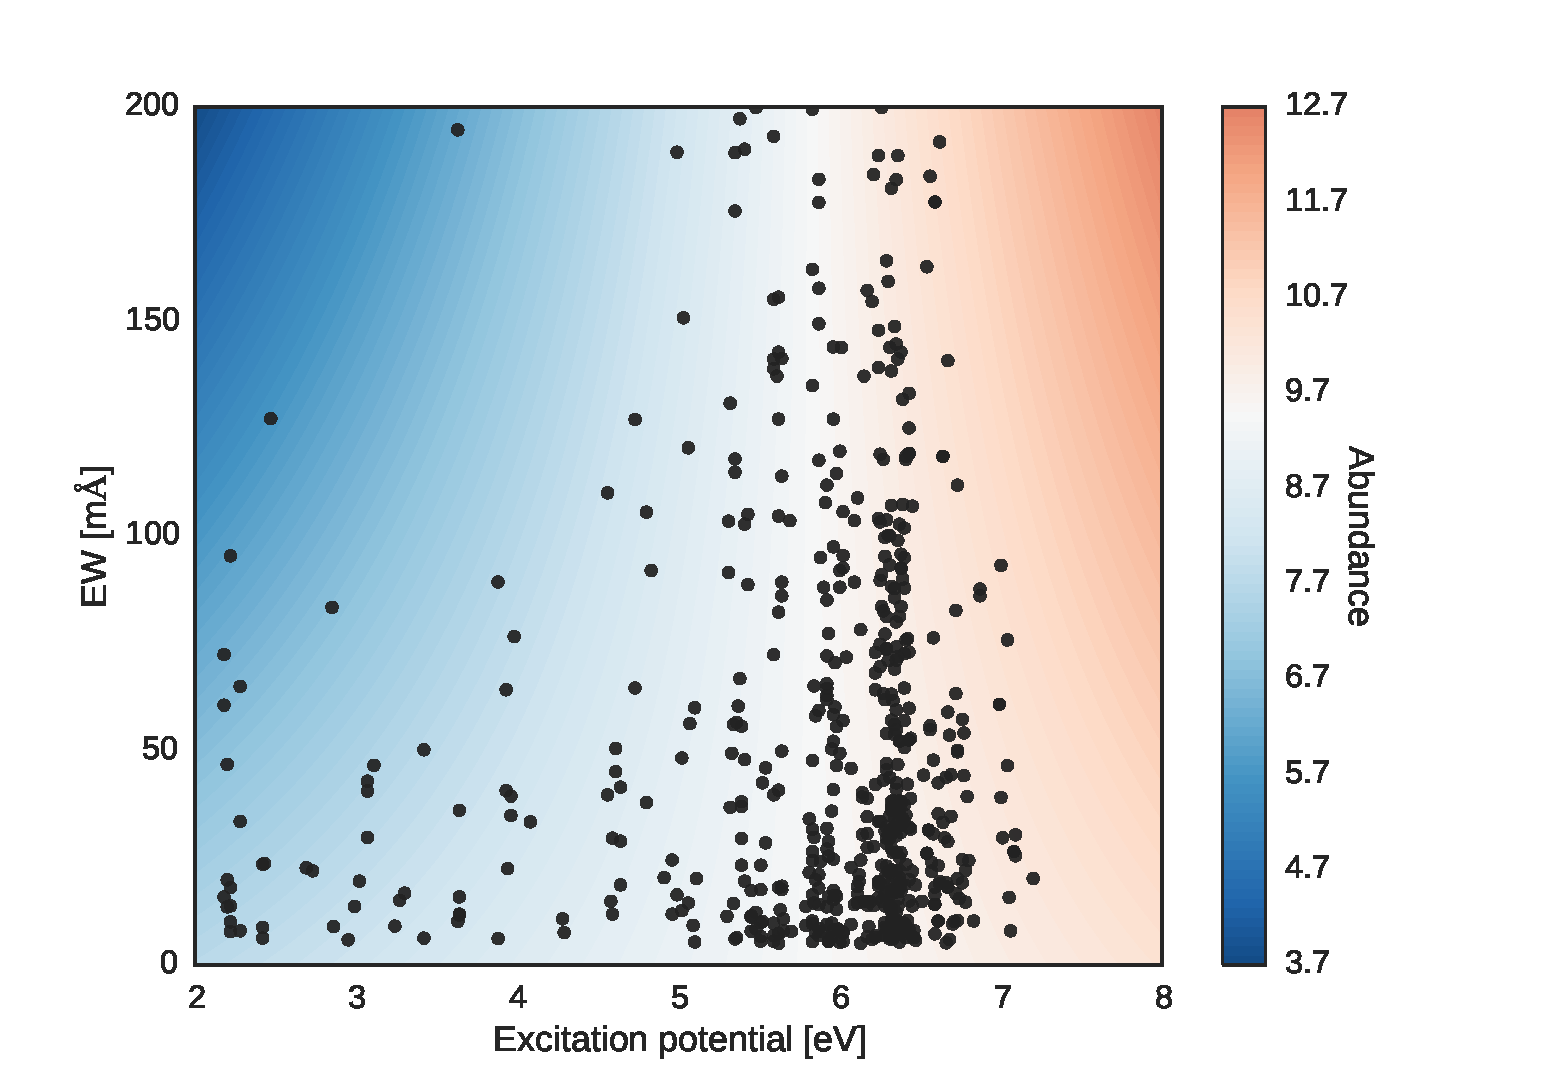
\includegraphics[width=0.9\linewidth]{figures/EWvsEP.pdf}
    \caption{The distribution of Fe I lines with. At the x axis is the
    excitation potential, while the measure EW is shown at the y axis. The
    color scale indicates the abundance before recalibration.}
    \label{fig:Fe1_before_recal}
\end{figure}


\begin{figure}[htpb]
    \centering
    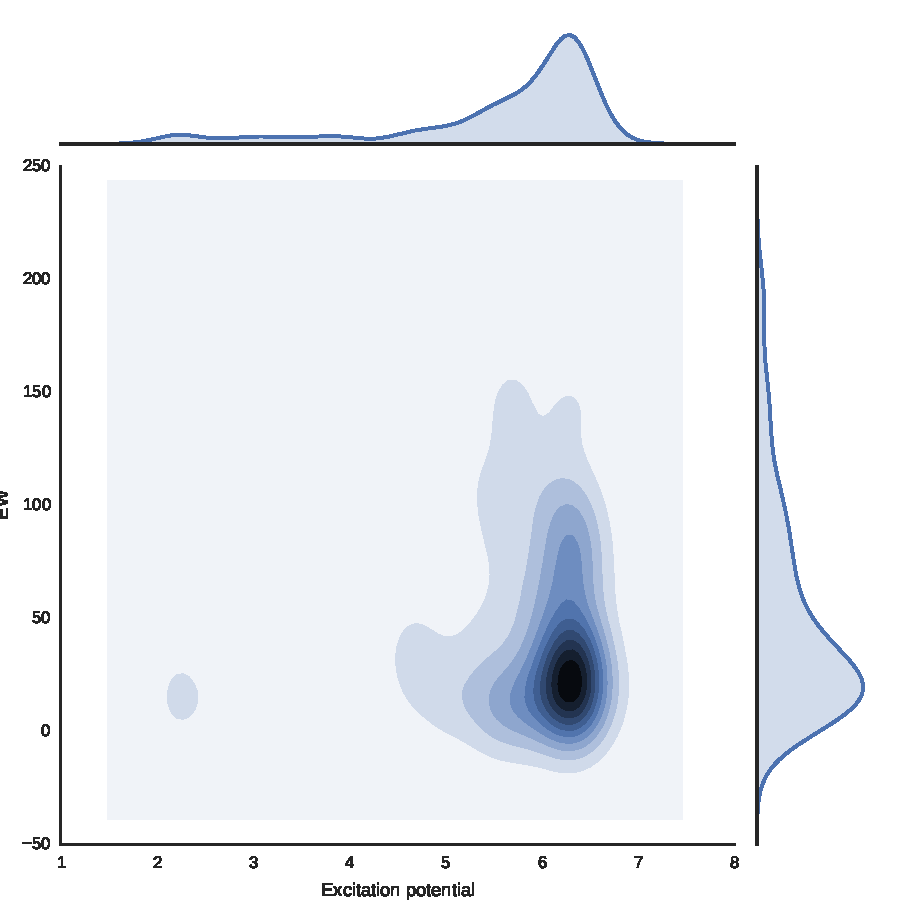
\includegraphics[width=0.9\linewidth]{figures/EWvsEP_cut.pdf}
    \caption{The distribution of Fe I lines. At the x axis is the
    excitation potential, while the measure EW is shown at the y axis.
    The histograms at the top and to the right of the plot, show the
    distribution of the respective axis.}
    \label{fig:Fe1_after_recal}
\end{figure}



\subsection{Deriving parameters with the EW method}
\label{sec:deriving_parameters_with_the_ew_method}

Once the EW's have been measured for all lines in the line list (or as
many as possible), the next step is to derive atmospheric parameters.
Atmosphere models are necessary for computing abundances of the lines.
The literature offers the possibility to choose from a wide variety
of model atmospheres. Models like ATLAS9 \citep{Kurucz1993} and
MARCS \citep{Gustafson2008} are the most used atmospheric models for
derivation of spectroscopic parameters for FGK stars.

Here we use the ATLAS9 models which, for efficiency, is created in
a grid according to effective temperature, surface gravity, and
metallicity. In order to search for final parameters it is necessary to
interpolate models from the grid, thus allowing to look in a finer grid
space.

For a given atmosphere model, abundances of all the lines in the line
list are calculated. By removing any correlation between the excitation
potential and abundance of all lines (from same element) the effective
temperature is constrained. In a similar way, the micro turbulence can
be constrained be removing any correlation between the reduced EW ($\log
EW$) and abundances, and the surface gravity is found when there is
ionization balance, i.e. the mean abundance of FeI and FeII are equal.
Lastly, the iron abundance comes from calculating the mean of
all the iron abundances.

When there are no longer any correlation, the final atmospheric
parameters are obtained from the atmospheric model to calculate the
given abundances.

In order to find the best atmosphere model, a minimization algorithm
is used based on the downhill simplex method \citep{Press1992} that
searches in the parameter space for the best fitting model. The
convergence criteria for the correlation between excitation potential
and abundances gives a slope less than 0.001, a slope less than 0.002
for the correlation between the reduced EW and the abundances, and a
difference of less than 0.005 between the mean abundances for FeI and
FeII.







\section{Results}
\label{sec:results}


\subsection{Derived parameters for the Sun}
\label{sec:derived_parameters_of_the_sun}

We derive atmospheric parameters for the Sun with the recalibrated line
list. This is a trivial case since the line list is calibrated for the
Sun, but it serves as a consistency test. Additionally, we added noise
to the EW measurements and derived parameters with different cuts in
excitation potential (EP). The noisy EW's follow the procedure from
\cite{Caryel1988}:

\begin{align}
    \sigma \simeq 1.6 \frac{\sqrt{\Delta\lambda EW}}{SNR},
\end{align}
where $\Delta\lambda=0.1$ and we consider to different signal-to-noise ratios,
100 and 300. This sigma is used to create a normal distribution with a mean
around the original EW.

\begin{align}
    f(x, EW, \sigma) = \frac{1}{\sqrt{2\pi\sigma^2}} e^{-\frac{(x-EW)^2}{2\sigma^2}}
\end{align}
A new EW is drawn from this distribution and the atmospheric parameters
are derived again. For all EWs we make 10 draws which corresponds to
20 different line lists (2 for each SNR we consider with 10 draws
each). For this 20 line lists we cut in the EP. The cuts are located
at $\SI{5.5}{eV}$ and $\SI{5.0}{eV}$. This gives additionally 40 line
lists, which is a total of 61 including the original line list which at
this point is used as a standard. We derive parameters for all 61 line
lists.


In Figure~\ref{fig:solar_parameters} the parameters are plotted with
different EP cuts in the line list. The horizontal black line is the
derived atmospheric parameters without noise added to the EW. This agree
well with solar values (ADD REFERENCE HERE). The color shows the two different
SNR considered.

\begin{figure}[htpb]
    \centering
    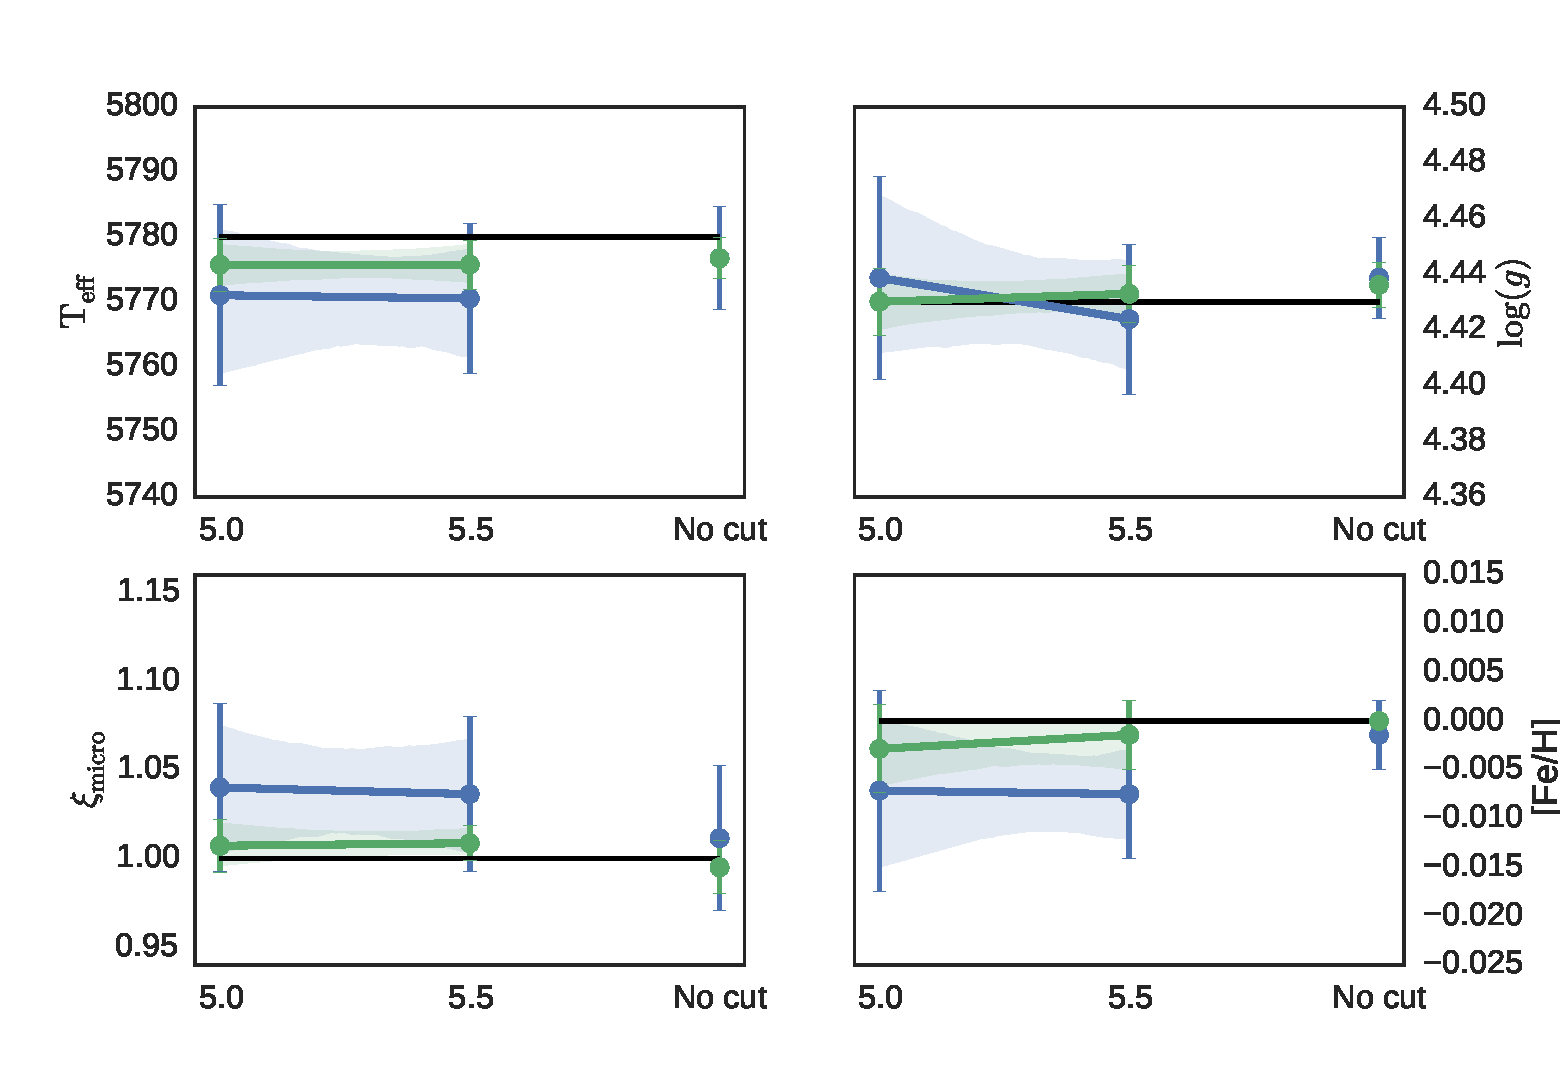
\includegraphics[width=0.9\linewidth]{figures/solar_parameters_10runs.pdf}
    \caption{Derived atmospheric parameters for the Sun. The horizontal
    black lines are the parameters for the calibrated line list, the
    three points shows the median value of 10 runs with random noise
    added, the blue points is the results for SNR=100, while the
    green points is for SNR=300.}
    \label{fig:solar_parameters}
\end{figure}

By adding noise to the EW measurements and calculate the atmospheric
parameters with different cuts in EP, we see how we over estimate all
the parameters except the iron abundance, when a cut in EP is not
applied. This suggest that it might be necessary to do a cut in the line
list for other stars to get reliable parameters. This is indeed the case
for HD20010.

The derived atmospheric parameters are presented in Table~\ref{tab:sun}.


\begin{table*}[htb!]
    \caption{The derived parameters for the Sun with two different cuts
    in EP, and with no cut. For all the line lists here, there is noise
    added to the EW measurements.}
    \label{tab:sun}
    \centering
    \begin{tabular}{lllll}
      \hline\hline
        EP cut (eV) & $T_\mathrm{eff}$ (K) & $\log g$ (cgs) & $\xi_\mathrm{micro}$ (km/s) & [Fe/H] \\
      \hline
        No cut      & 5920 \pm 247         & 4.94 \pm  0.64 & 4.99 \pm 3.96               & -0.03 \pm 0.14\\
        5.0         & 5738 \pm 274         & 4.54 \pm  0.72 & 4.99 \pm 4.83               & -0.11 \pm 0.25\\
        5.5         & 5612 \pm 158         & 4.49 \pm  0.70 & 4.80 \pm 5.64               & -0.24 \pm 0.44\\
      \hline
    \end{tabular}
\end{table*}




\subsection{Derived parameters for HD20010}
\label{sec:derived_parameters_of_hd20010}

HD20010 is a well studied F8 subgiant, see e.g.
\cite{Mortier2013,Lebzelter2012}. Therefore, it is a prime object for
our studies, since we want to benchmark results from our new line list
with literature values. To analyse this star we used spectra from
the CRIRES-POP \citep{Lebzelter2012}. The data comes in pieces of
$\SI{50}{\angstrom}$ to $\SI{120}{\angstrom}$. At the time of writing
the data is not yet fully reduced. This is a task the CRIRES-POP team
is working on. However, the data can still be used as it is after the
pipeline reduction. It is already known by the CRIRES-POP team that the
pipeline reduced form of the wavelength calibration is of poor quality.
Most of the spectra are stretched compared to e.g. a model or a solar
spectrum in the same region.

In order to measure the EW of the lines in our line list, the correct
absorption lines need to be identified. This was done by plotting
the spectra for HD20010, a solar spectrum (the parameters are close
enough so we can use the Sun as a reference), an observed telluric
spectrum from the TAPAS web page \citep{Bertaux2014}, and the lines from our
line list in the region we are looking at. The pieces of spectra are
shifted in radial velocity as well. A software was developed that plots
everything and calculate the cross correlation function of the model
(in this case the Sun), and the telluric spectra\footnote{The software
(plot\textunderscore{}fits) is open source and can be found here:
\url{https://github.com/DanielAndreasen/astro_scripts}}. The two CCFs
are fitted with a Gaussian, and the mid point is the RV. This two, in
principle, different radial velocities shift the model and the telluric
spectra. The lines from our line list are shifted with the same RV as for
the model. Figure~\ref{fig:plot_fits} shows an example of this.

\begin{figure}[htbp!]
    \centering
    \includegraphics[width=0.9\linewidth]{figures/plot_fits.pdf}
    \caption{The middle plot shows a piece of HD20010 (black), the model
    spectrum, in this case the Sun (green), a telluric spectrum (red), and two
    lines from our line list (magenta vertical lines). The plot to the left
    shows the CCF of the Sun with a fitted Gaussian. The right plot shows the
    same as the one to the left, but for the telluric spectrum.}
    \label{fig:plot_fits}
\end{figure}

The derived parameters for HD20010 for the full line list
are overestimated compared to literature values, see e.g.
\citet{Mortier2013,Lebzelter2012}. To overcome this problem we tried
to remove lines above different EPs and re-determine the atmospheric
parameters. In this process we did not remove any of the FeII
lines (we were only able to measure the EW of 5 lines out of the
13 from the solar case). In the line list by \cite{Tsantaki2013}
covering a visual range the maximum EP is $\SI{5.1}{eV}$.
Figure~\ref{fig:HD20010_parameters_cuts} shows the results from this
exercise. In the minimization process the surface gravity were fixed
at 4.11(ADD REFERENCE) in order to reach convergence. This is a mean
value of previous studies. A second degree polynomial is fitted for the
effective temperature, iron abundance, and the micro turbulence with
the 95\% confidence interval. At a cut at $\SI{5.5}{eV}$ and below the
atmospheric parameters gets closer to the literature values which is
plotted as a horizontal black line. The exact values can be seen in
Table~\ref{tab:hd20010}.

\begin{table*}[htb!]
    \caption{The derived parameters for HD20010 at different EP cut. $\log g$
    were fixed at 4.11 for all calculations.}
    \label{tab:hd20010}
    \centering
    \begin{tabular}{lllll}
      \hline\hline
        EP cut (eV) & $T_\mathrm{eff}$ (K) & $\xi_\mathrm{micro}$ (km/s) & [Fe/H] \\
      \hline
      5.0           & 6098                 & 0.67                        & -0.22   \\
      5.1           & 6060                 & 1.31                        & -0.26   \\
      5.2           & 6084                 & 1.29                        & -0.25   \\
      5.3           & 6081                 & 1.29                        & -0.25   \\
      5.4           & 6149                 & 2.01                        & -0.27   \\
      5.5           & 6324                 & 2.05                        & -0.23   \\
      5.6           & 6353                 & 2.12                        & -0.23   \\
      5.7           & 6596                 & 2.10                        & -0.18   \\
      5.8           & 6601                 & 2.10                        & -0.18   \\
      5.9           & 6992                 & 2.02                        & -0.09   \\
      6.0           & 7000                 & 2.03                        & -0.08   \\
      No cut        & 7138                 & 2.87                        & -0.06   \\
      \hline
    \end{tabular}
\end{table*}


\begin{figure}[htpb!]
    \centering
    \includegraphics[width=0.9\linewidth]{figures/HD20010_parameters_cuts.pdf}
    \caption{Atmospheric parameters for HD20010. In the top panel is the
    effective temperature. The middle panel is the iron abundance, and the
    bottom panel is the micro turbulence. The parameters are derived with
    different cuts in EP. Here the horizontal black lines are literature values.
    The parameters for the full line list are plotted to the right for all
    three plots.}
    \label{fig:HD20010_parameters_cuts}
\end{figure}











\newpage
\bibliography{thesis}
\bibliographystyle{astron}
\nocite*{}

\end{document}
